\section{Redox-Reaktionen}

\subsection{Definition}
\begin{tabular}{l l}
	Oxidationsmittel \textbf{(OM)} & der Stoff, der Elektronen aufnimmt                  \\
	                               & und \textbf{reduziert} wird ($+e^-$)                       \\
	Reduktionsmittel \textbf{(RM)} & der Stoff, der die Elektronen abgibt                \\
	                               & und \textbf{oxidiert} wird ($-e^-$)                        \\
\end{tabular}

\subsection{Redox Reaktionsgleichung - Ablauf}

\begin{enumerate}
	\item \textbf{Findet eine Reaktion überhaupt statt?} \\
	Man liest die Redoxreihe von \textbf{links nach rechts}. \\
	Eine \textbf{oxidierte Form} reagiert mit einer \textbf{reduzierten Form}, die \textbf{unter ihr} in der Redoxreihe steht – das nennt man eine \textit{Bergab-Stellung}.
	
	\item \textbf{Edukte} kommen auf die \textbf{linke Seite}, \textbf{Produkte} auf die \textbf{rechte Seite} der Reaktionsgleichung.
	
	\item \textbf{Oxidationszahl} nachsehen:
	\begin{itemize}
		\item Um zu erkennen, wie viele \textbf{Elektronen ein Stoff abgibt oder aufnimmt}
		\item Das zeigt, welche \textbf{Valenzelektronen bindungsfähig} sind (Ladungen).
		\item Das \textbf{Elektronennegativere} übernimmt die Elektronenladung (z.\,B.\ \ch{C} bei einer \ch{C-H}-Bindung).
	\end{itemize}
	
	\item \textbf{Ausgleichen} der Reaktionsgleichung (Elektronen-, Massen- und Ladungsausgleich).
\end{enumerate}

\begin{flushleft}
	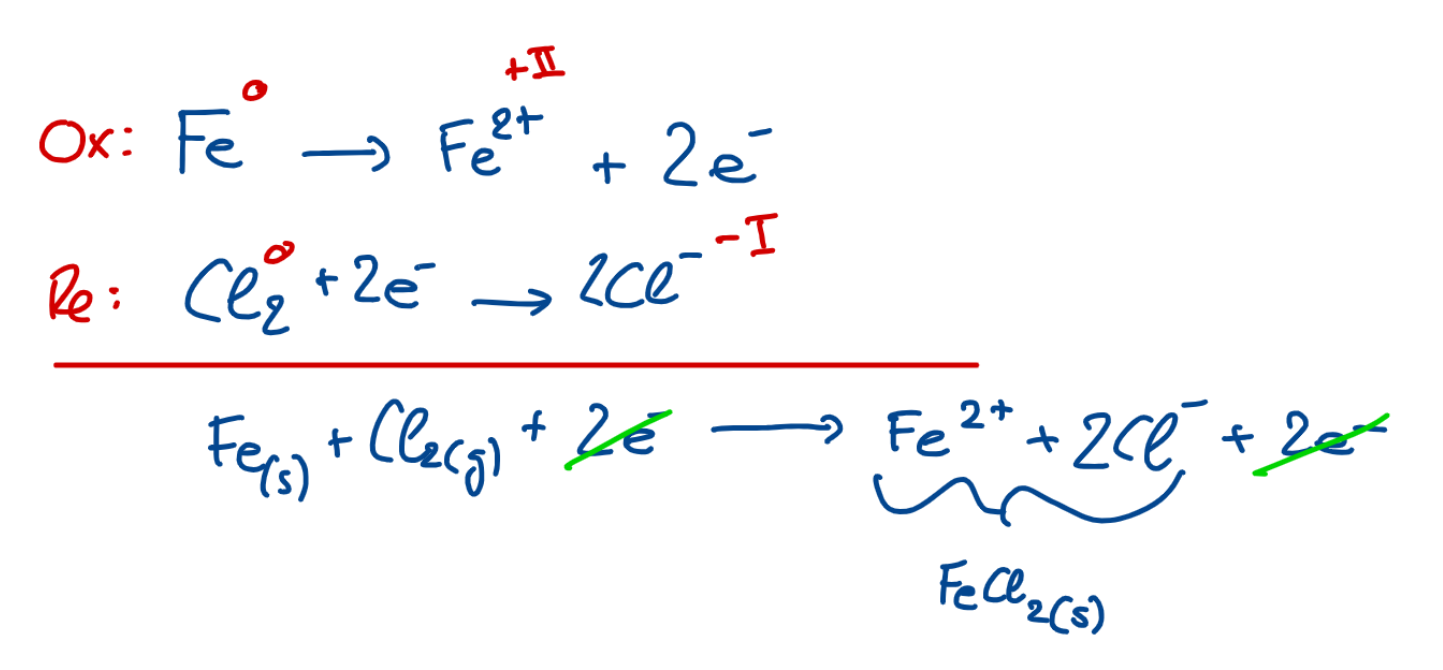
\includegraphics[width=0.5\linewidth]{images/redoxreaktion.png}
\end{flushleft}